\presec \vvv
\section{Optimizations: Final Version} \postsec
\label{sec:optimization}
\label{sec:final}

To address the two shortcomings of our basic version, we propose an optimization method. 
For convenience, and without loss of generality, \textit{we assume the interest is frequency in this section}. When interest is defined as change of frequency, persistency or connection, the optimization remains unchanged. 
%In practice, we recommend using our final version of storing multiple items in one bucket, because it overcomes all shortcomings of the previous versions.
%(see Section \ref{sec:final}).
%^and related experiments are shown in Appendix~\ref{eva_para}.


\begin{comment}

%\presub \vvv\vvv
%\subsection{Using Stream-Summary}
\postsub

The basic version of our algorithm is slow with insertions. 
%
To address this, we accelerate our algorithm by replacing the min-heap with Stream-Summary\cite{spacesaving} and a hash table. 
%
Stream-Summary is a data structure proposed by the authors of SpaceSaving~\cite{spacesaving}. 
%
It can achieve $O(1)$ time complexity for both updating the heap and returning the smallest item. 
%
Stream-Summary is a double-directional linked list consisting of nodes.
%
Each node stores a unique frequency. 
%
For a given node with frequency $f$, it has a linked list storing all the items whose frequency is exactly $f$.
%
In the hash table, the key is the flow ID, and the value is a pointer to the corresponding node in the min-heap.
%
The hash table is used to check whether the incoming flow is in the Stream-Summary, and if so, the corresponding frequency will be incremented by 1.


However, this optimization has inevitable drawbacks.
%
First, Stream-Summary consumes a relatively large amount of memory, since it is a double-directional linked list and each node has four or six pointers. 
%
Second, the hash table also requires a significant amount of memory space to minimize the hash collision rate. 
%
Third, the update process is relatively slow because multiple pointers need to be modified for each update.
\end{comment}

\begin{comment}
\presub
\subsection{Using Multiple Arrays} \postsub
\label{sec:multi:array}

To solve the problem of memory space consumption in the previous optimization, we propose another optimization using multiple arrays. 

\begin{figure}[htbp]
	\centering
	\prefig
	%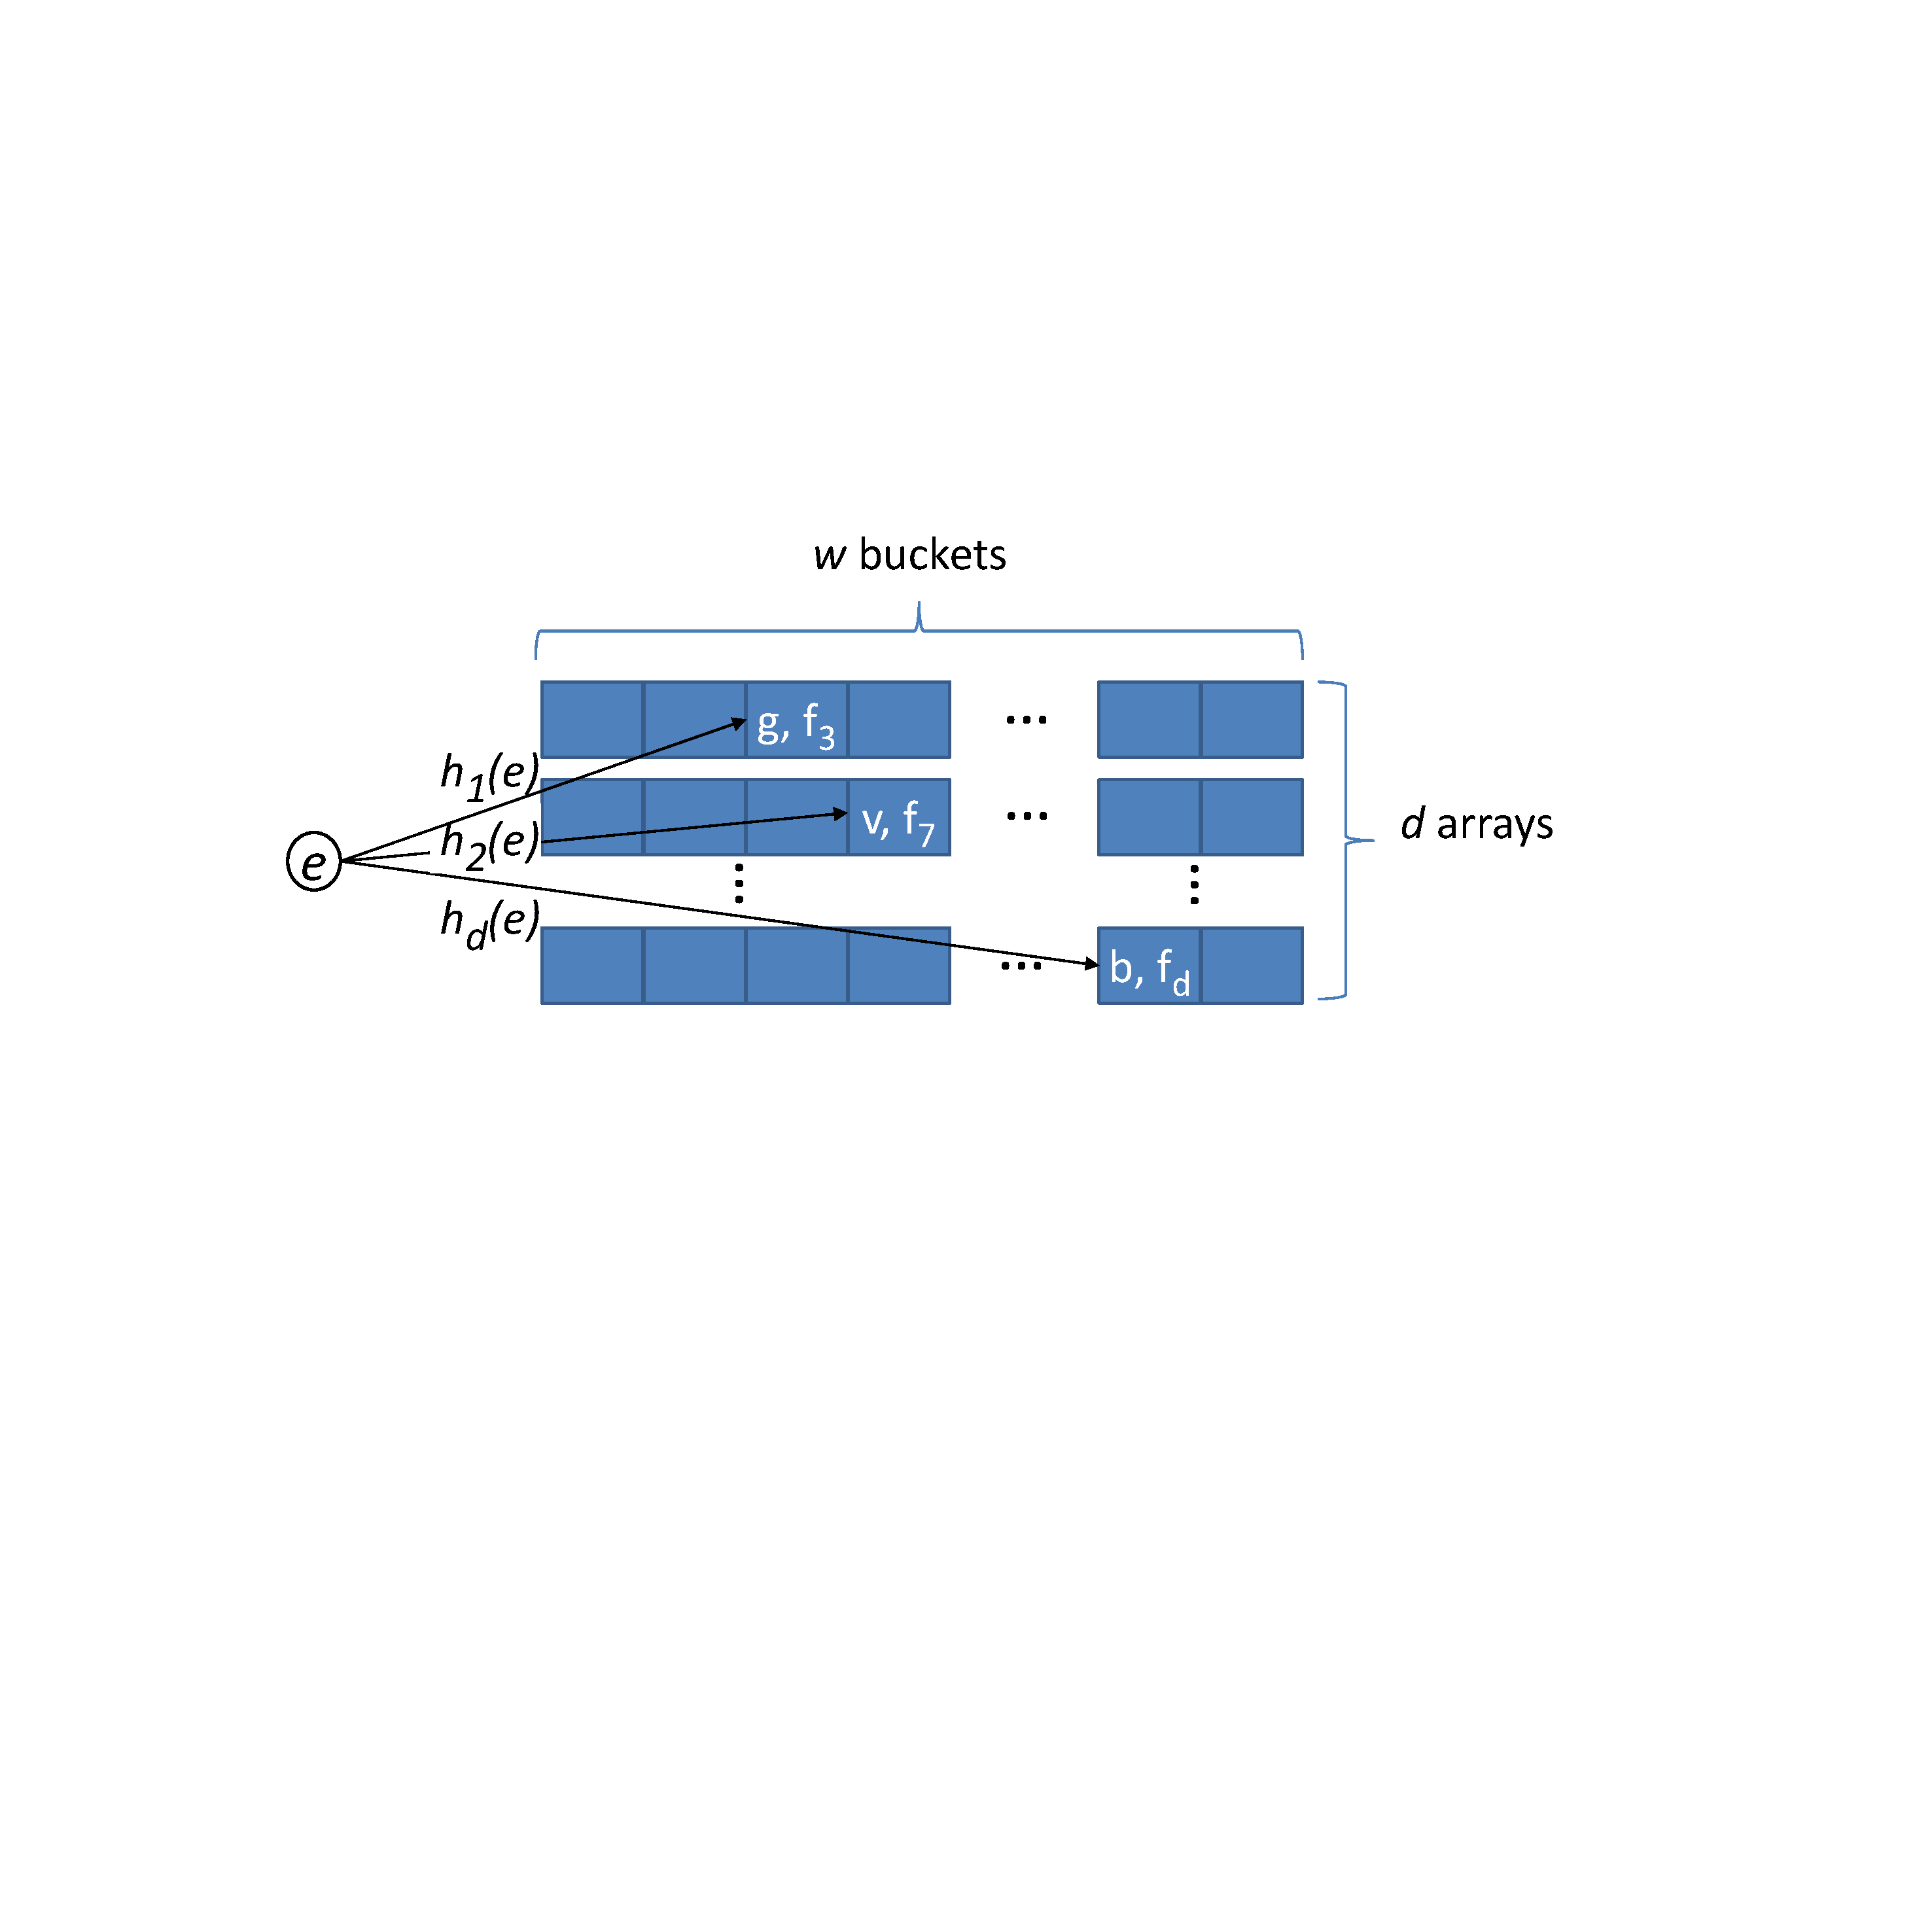
\includegraphics[width=0.49\textwidth]{mul_array}
	\prefigcaption
	\caption{\aname{} using multiple arrays.}
	\label{draw:mul_array}
	\postfig
\end{figure}

\ppp{Data Structure (Figure~\ref{draw:mul_array}):}
There are $d$ arrays in total and each array corresponds to a hash function. 
%
Each array consists of $w$ buckets and each bucket stores the ID and frequency of an item. Every bucket has its own $t_{fail}$.

\ppp{Insertion:}
%For an incoming item $e$, we calculate $d$ hash functions and pick the corresponding $d$ buckets.
%
There are three cases. First, if one of the $d$ buckets stores the item with the same ID as the incoming item $e$, we increment the frequency in that bucket. 
%
Second, if there is no item with the same ID as $e$ but there are empty buckets, we just store $e$ in the first empty bucket. 
%
Third, if there is neither item with the same ID nor empty buckets, we select the bucket with the smallest frequency and replace the original item with the incoming one using our PRI algorithm. 

 \ppp{Query:}
 For a given item $e$, to find its frequency, we just calculate $d$ hash functions and pick out the corresponding $d$ buckets.
% %
 If there is an item with the same ID as $e$ in any one of the $d$ buckets, the frequency stored in that bucket is returned. Otherwise, we report false.

\ppp{Report:}
%To return the items with frequency larger than a predefined threshold $\mathcal{T}$, we traverse the $d$ arrays. 
%
If the frequency stored in a bucket is larger than $\mathcal{T}$, the corresponding item is reported.

 \ppp{Deletion:}
 Given the ID of an item, to delete that item from our data structure, we calculate $d$ hash functions. If the item with the same ID exists, we decrement the frequency by one. Otherwise, the data structure remains unchanged.

\ppp{Advantages and Disadvantages:}
Compared with the memory hungry Stream-Summary, using multiple arrays minimizes the memory usage thanks to the following two reasons.
%
First, there is no pointer in this data structure. Second, since the number of items is far larger than that of buckets, there are few, if any, empty buckets.
%
Given the same memory space, using multiple arrays outperforms Stream-Summary to a large extent in terms of accuracy.  
%
However, the time complexity of insertions is $O(d)$, where $d$ is the number of arrays. 
%
Although $d$ can be small (\eg, 3 or 4), we still wish to reduce the time complexity to $O(1)$, without sacrificing accuracy or memory efficiency. 
%
Therefore, we propose the final optimization in the following subsection.
\end{comment}

%\presub\vvv
%\subsection{Final Version: Storing Multiple Items in one Bucket} \postsub

%\ppp{Final Version: Storing Multiple Items in one Bucket}
%We recommend this final version for finding interesting items, because it overcomes all shortcomings of the previous versions.
 
 \begin{figure}[htbp]
	\centering
	\prefig \vspace{-0.05in}
	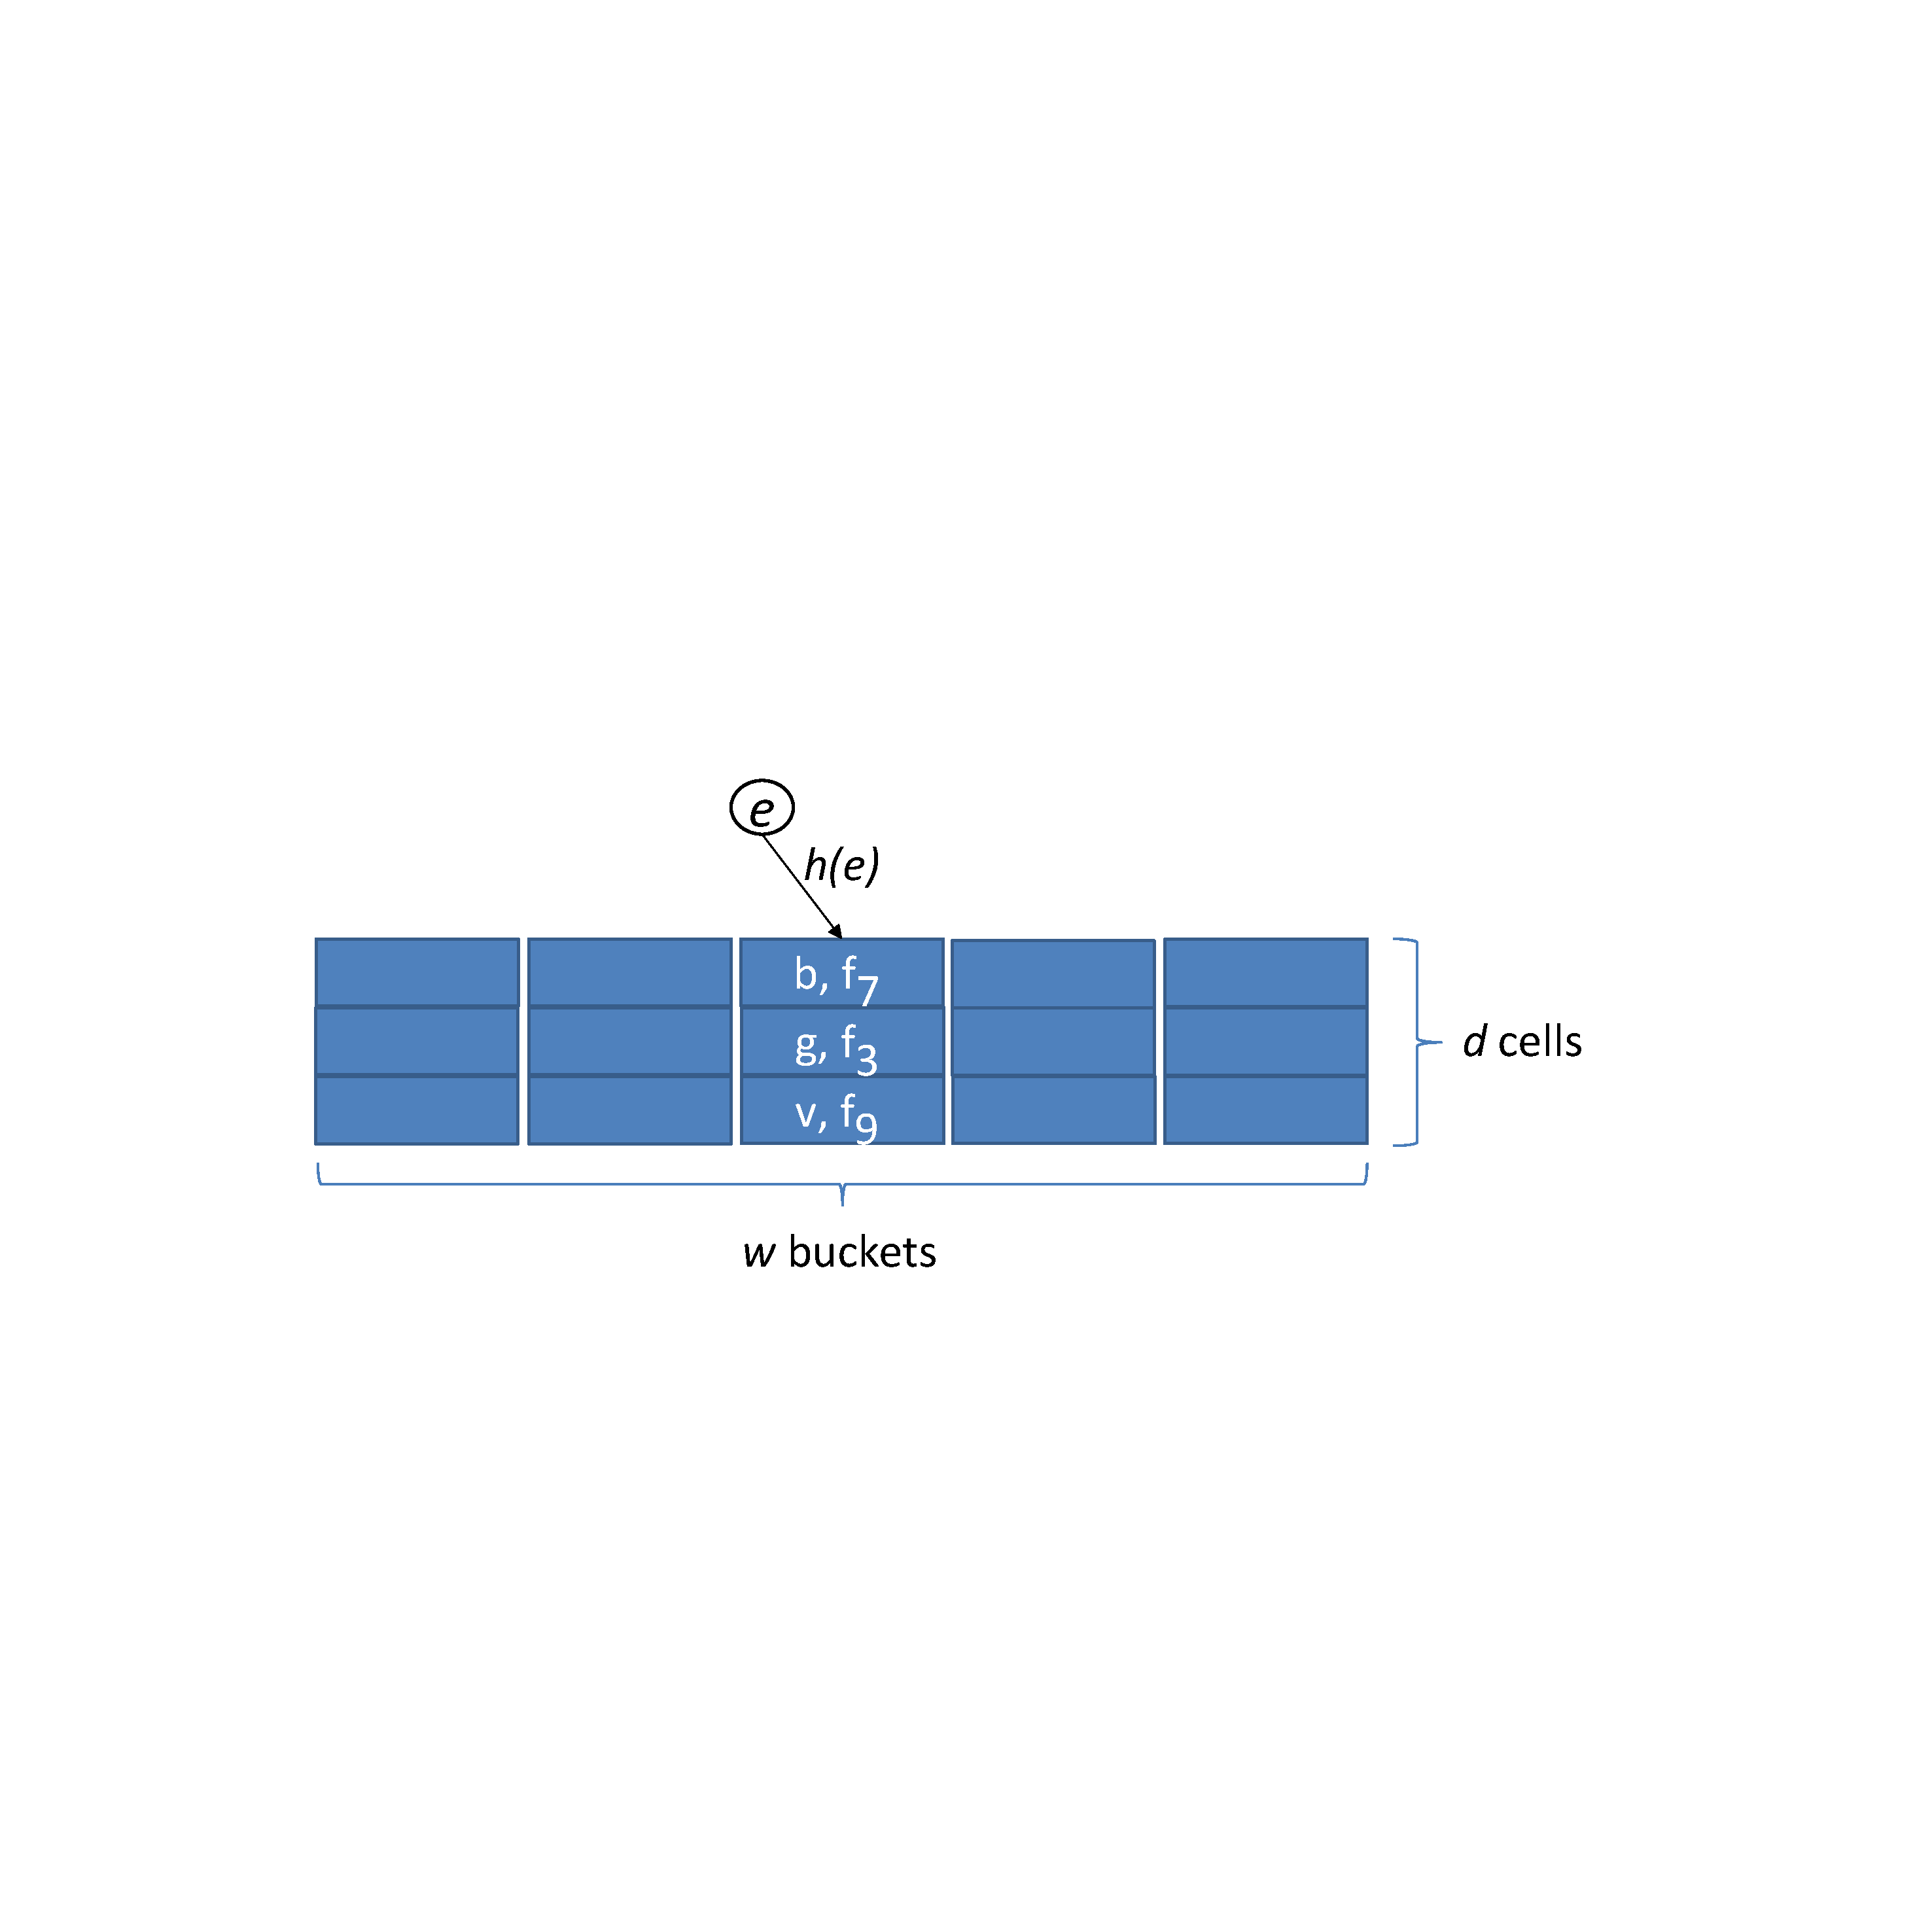
\includegraphics[width=0.48\textwidth]{mul_cell}
	\prefigcaption \vspace{-0.05in} \vspace{-0.05in}
	\caption{\aname{} using multiple cells in every bucket.}
	\label{draw:mul_cell}
	\postfig \vspace{-0.05in}
\end{figure}

\ppp{Data Structure:}
As shown in Figure~\ref{draw:mul_cell}, there is one array which consists of $w$ buckets. 
%
Each bucket has $d$ cells storing the ID and frequency of an item. Every bucket has also its own $t_{fail}$.

\ppp{Insertion:}
Given an incoming item $e$, we calculate the hash function and pick the corresponding bucket.  
%
There are three cases. First, if one of the items in the bucket has the same ID as the incoming item $e$, we increment the frequency of that item by 1. 
%
Second, if there is no item with the same ID as $e$ but the bucket is not full, we store $e$ in the first empty cell in that bucket. 
%
Third, if there is no item with the same ID nor empty cell, we select the item $e_{min}$ with the smallest frequency $f_{min}$ in the corresponding bucket and replace $e_{min}$ with the incoming one $e$ using our PRI algorithm: we replace $e_{min}$ with the item $e$ with a probability of $1/(2f_{min}-t_{fail}+1)$. If replacing is successful, we increment the frequency from $f_{min}$ to $f_{min}+t_{fail}/f_{min}$. Otherwise, the frequency remains unchanged. 

% \ppp{Query:}
% For a given item $e$, to find its frequency, we just calculate the hash function and pick out the corresponding bucket with $d$ cells. 
% %
% If there is an item with the same ID as $e$ in one of the $d$ cells, the frequency stored in that cell is returned. Otherwise, we report false.

\ppp{Report:}
To return the items with frequency larger than a predefined threshold $\mathcal{T}$, we traverse the $w$ buckets and $d$ cells in each bucket, and report all appropriate items. 

%If the frequency stored in a cell in any bucket is larger than $\mathcal{T}$, the corresponding item is reported.

% \ppp{Deletion:}
% Given the ID of an item, to delete that item from our data structure, we calculate the hash function and pick out the corresponding bucket.
% %
% Then all cells in that bucket is traversed. 
% %
% If the item with the same ID exists in any cell, we decrement the corresponding frequency by one.
% %
% Otherwise, we report that the item does not exist.


\ppp{Analysis:}        
The final version has the following advantages.
%
First, this data structure has high memory efficiency, since it neither applies pointers nor has many empty cells. Second, by applying our PRI algorithm, it reaches a much higher accuracy compared with SpaceSaving. 
Third, the time complexity for processing each packet is reduced to $O(1)$, because each insertion only needs to probe one bucket.
%
%The algorithm is shown in Algorithm~\ref{alg:mul}.


\begin{comment}
\begin{algorithm}
	%	\SetLine
	\KwIn{An item $e_i$}
	$random()\in [0,1]$\\
	$b_i \gets b[h(e_i)\%w]$\;
	\eIf{$e_{i}\in b_i$}
	{
		$Interest(e_{i})++$\;
	}
	  {
        \eIf{$b_i$ has empty cells }
	        {
	        $b_i.insert(e_{i})$\;	
	        }
	   {
	       \eIf{$random() \leqslant \frac{1}{2*\iii_{min}-
t_{fail}+1}$}
              {
	           $e_{min} \gets e_i$\;
	           $\iii_{min} \gets \iii_{min} + \frac{t_{fail}}{\iii_{min}}$\;
	           $t_{fail} \gets 0$\;
	          }
	          {
	          $t_{fail}++$\;
	          }
	   }
	  }
	\caption{Insertion process for the final version.}
	\label{alg:mul}
\end{algorithm}

\end{comment}



